\documentclass[tikz,border=2pt]{standalone}
\usepackage{fontspec}
\setmainfont{Inter}[BoldFont={Inter SemiBold}]
\setmonofont{JetBrains Mono}
\providecommand\theme{light}
\def\darktheme{dark}
\ifx\theme\darktheme
  \definecolor{fg}{HTML}{E6EDF8}\definecolor{muted}{HTML}{9AA8C2}
  \definecolor{panel}{HTML}{0C1730}\definecolor{chip}{HTML}{0F1C38}
  \definecolor{line}{HTML}{1E2D4D}\definecolor{accent}{HTML}{4D9BFF}
  \definecolor{newfill}{HTML}{12305F}\definecolor{onaccent}{HTML}{070F1F}
\else
  \definecolor{fg}{HTML}{0E1A33}\definecolor{muted}{HTML}{51607A}
  \definecolor{panel}{HTML}{F4F7FC}\definecolor{chip}{HTML}{FFFFFF}
  \definecolor{line}{HTML}{DDE4F0}\definecolor{accent}{HTML}{0F66E0}
  \definecolor{newfill}{HTML}{E3EEFF}\definecolor{onaccent}{HTML}{FFFFFF}
\fi

\tikzset{
  panel/.style={draw=line, fill=panel, rounded corners=6pt, line width=0.8pt},
  title/.style={anchor=north west, inner sep=0, text=fg, font=\bfseries\fontsize{9}{11}\selectfont},
  chip/.style={anchor=north west, draw=line, fill=chip, rounded corners=4pt, line width=0.7pt,
               minimum height=0.62cm, text height=1.55ex, text depth=0.45ex, text width=#1, inner xsep=7pt, align=left, text=fg,
               font=\ttfamily\fontsize{7.8}{9}\selectfont},
  new/.style={draw=accent, fill=newfill, line width=1pt},
  badge/.style={anchor=east, rounded corners=5pt, inner xsep=4pt, inner ysep=1.6pt,
                font=\bfseries\fontsize{6}{7}\selectfont},
  newbadge/.style={badge, fill=accent, text=onaccent},
  betabadge/.style={badge, draw=accent, line width=0.7pt, text=accent},
}
% \modgroup{x}{y}{width}{height}{title}
\newcommand\modgroup[5]{\draw[panel] (#1,#2) rectangle ++(#3,-#4);
  \node[title] at ($(#1,#2)+(0.3,-0.3)$) {#5};}
\usetikzlibrary{calc}
\begin{document}
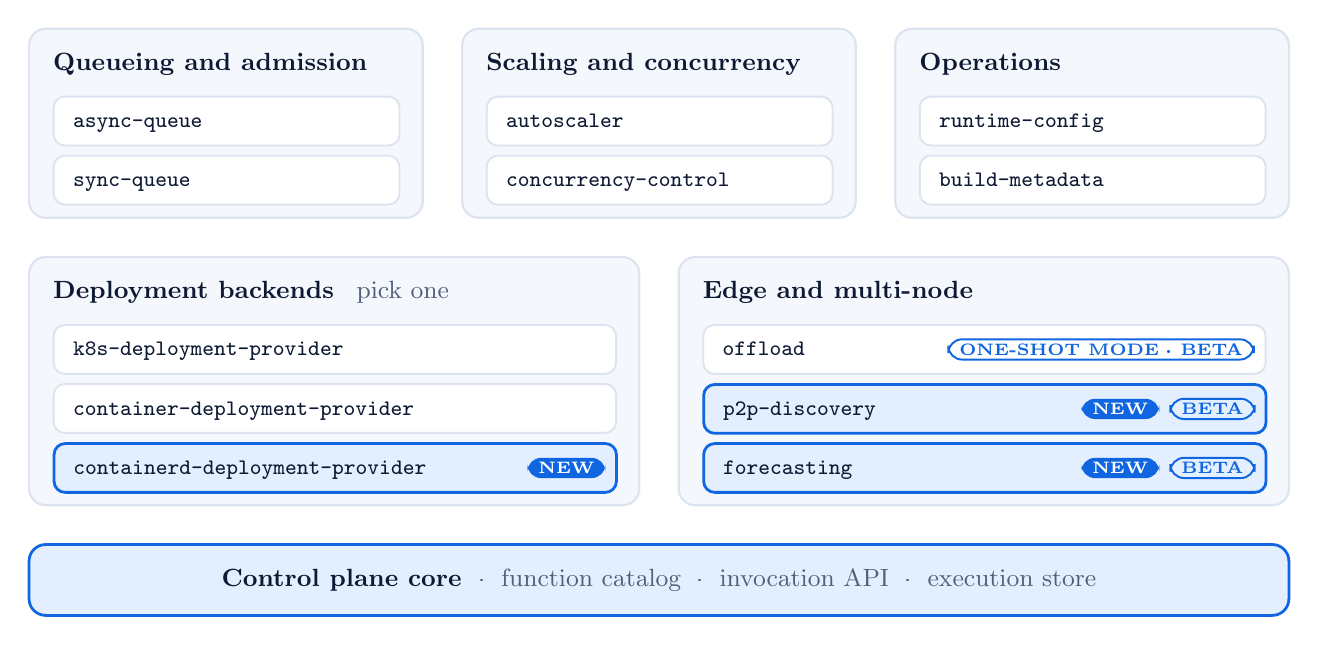
\begin{tikzpicture}
  % top row: three panels 5.0 wide, 2.4 high
  \modgroup{0}{0}{5.0}{2.4}{Queueing and admission}
  \node[chip=3.9cm] at (0.3,-0.85) {async-queue};
  \node[chip=3.9cm] at (0.3,-1.6) {sync-queue};

  \modgroup{5.5}{0}{5.0}{2.4}{Scaling and concurrency}
  \node[chip=3.9cm] at (5.8,-0.85) {autoscaler};
  \node[chip=3.9cm] at (5.8,-1.6) {concurrency-control};

  \modgroup{11}{0}{5.0}{2.4}{Operations}
  \node[chip=3.9cm] at (11.3,-0.85) {runtime-config};
  \node[chip=3.9cm] at (11.3,-1.6) {build-metadata};

  % bottom row: two panels 7.75 wide, 3.15 high
  \modgroup{0}{-2.9}{7.75}{3.15}{Deployment backends \textcolor{muted}{\mdseries\, pick one}}
  \node[chip=6.65cm] at (0.3,-3.75) {k8s-deployment-provider};
  \node[chip=6.65cm] at (0.3,-4.5) {container-deployment-provider};
  \node[chip=6.65cm, new] (cd) at (0.3,-5.25) {containerd-deployment-provider};
  \node[newbadge] at ($(cd.east)+(-0.15,0)$) {NEW};

  \modgroup{8.25}{-2.9}{7.75}{3.15}{Edge and multi-node}
  \node[chip=6.65cm] (off) at (8.55,-3.75) {offload};
  \node[betabadge] at ($(off.east)+(-0.15,0)$) {ONE-SHOT MODE · BETA};
  \node[chip=6.65cm, new] (p2p) at (8.55,-4.5) {p2p-discovery};
  \node[betabadge] (b1) at ($(p2p.east)+(-0.15,0)$) {BETA};
  \node[newbadge] at ($(b1.west)+(-0.12,0)$) {NEW};
  \node[chip=6.65cm, new] (fc) at (8.55,-5.25) {forecasting};
  \node[betabadge] (b2) at ($(fc.east)+(-0.15,0)$) {BETA};
  \node[newbadge] at ($(b2.west)+(-0.12,0)$) {NEW};

  % core
  \draw[draw=accent, fill=newfill, rounded corners=6pt, line width=1pt] (0,-6.55) rectangle (16,-7.45);
  \node[text=fg, font=\bfseries\fontsize{9.5}{11}\selectfont] at (8,-7.0)
    {Control plane core \textcolor{muted}{\mdseries\;·\; function catalog \;·\; invocation API \;·\; execution store}};
\end{tikzpicture}
\end{document}
